% !TeX spellcheck = pl_PL
\documentclass[a4paper,twoside]{article}
\usepackage{polski}
\usepackage[utf8]{inputenc}
\usepackage{graphicx}
\usepackage{amsmath}

\usepackage[unicode, bookmarks=true]{hyperref} %do zakładek
\usepackage{tabto} % do tabulacji
\NumTabs{6} % globalne ustawienie wielkosci tabulacji
\usepackage{array}
\usepackage{multirow}
\usepackage{array}
\usepackage{dcolumn}
\usepackage{bigstrut}
\usepackage{color}
\usepackage[usenames,dvipsnames]{xcolor}
\usepackage{svg}
\usepackage{xfrac}
\usepackage{floatrow}
\usepackage{enumitem}
\usepackage{listings,lstautogobble}


\usepackage{multirow,tabularx}
\newcolumntype{Y}{>{\centering\arraybackslash}X}
\renewcommand{\arraystretch}{2}

% === Reset inkrementacji sekcji przy nowym parcie === %
\usepackage{titlesec}

\makeatletter
\@addtoreset{section}{part}
\makeatother
\titleformat{\part}[display]
{\normalfont\LARGE\bfseries\centering}{}{-60pt}{}

% === Dodanie krpki do sekcji
\titlelabel{\thetitle.\quad}


\setlength{\textheight}{24cm}
\setlength{\textwidth}{15.92cm}
\setlength{\footskip}{10mm}
\setlength{\oddsidemargin}{0mm}
\setlength{\evensidemargin}{0mm}
\setlength{\topmargin}{0mm}
\setlength{\headsep}{5mm}

\setlength{\textfloatsep}{10pt plus 1.0pt minus 2.0pt}


\begin{document}
	\bibliographystyle{plain}
	
	% ************************************************************
	% --- Strona tytułowa
	% ************************************************************
	\begin{titlepage}
		\begin{table}[htbp]
			\centering
			\begin{tabular}{|c|c|c|c|c|c|c|}
				\hline
				\multicolumn{7}{|c|}{\textbf{{\LARGE Grafika Komputerowa}}} \bigstrut\\[4pt]
				\hline
				Rok akademicki & Termin & Rodzaj studiów & Kierunek & Prowadzący & Grupa & Sekcja \bigstrut\\
				\hline
				\multicolumn{1}{|c|}{\multirow{2}[4]{*}{{\large 2014/2015}}} & \multicolumn{1}{c|}{{\large Piątek}} & \multicolumn{1}{c|}{\multirow{2}[4]{*}{{\large SSI}}} & \multicolumn{1}{c|}{\multirow{2}[4]{*}{{\large INF}}} & \multicolumn{1}{c|}{\multirow{2}[4]{*}{\begin{tabular}{@{}c@{}}{\large dr} \\[-9pt] {\large Ewa Lach}\end{tabular}}} & \multicolumn{1}{c|}{\multirow{2}[4]{*}{{\large GKiO3}}} & \multicolumn{1}{c|}{\multirow{2}[4]{*}{{\large 1}}} \bigstrut\\
				\cline{2-2}    \multicolumn{1}{|c|}{} & \multicolumn{1}{c|}{{\large 09:30 - 11:00}} & \multicolumn{1}{c|}{} & \multicolumn{1}{c|}{} & \multicolumn{1}{c|}{} & \multicolumn{1}{c|}{} & \multicolumn{1}{c|}{} \bigstrut\\
				\hline
			\end{tabular}%
		\end{table}%
		
		\centering
		
\includegraphics[width=0.6\textwidth]{./images/logo.png}
		\\\vspace{10mm}
		\textbf{{\huge Raport wersji Beta}}\\\vspace{5mm}
		\textbf{{\Huge Danmaku Shooter}}
		\\
		\vfill
		\begin{flushright}
			{\Large \textbf{Skład sekcji}:}\\
			\begin{tabular}{rr}
				{\Large Buchała} & {\Large Bartłomiej}\\[-3pt]
				{\Large Forczmański} & {\Large Mateusz}\\[-3pt]
				{\Large Motyka} & {\Large Marek}\\[-3pt]
				{\Large Wudecki} & {\Large Wojciech}
			\end{tabular}
		\end{flushright}
	\end{titlepage}
	
	\newpage
	\part{Realizacja zadań}
		\section{Interfejs gracza}
			W pełni zrealizowany. Na ekranie widoczne są wszystkie informacje potrzebne dla gracza jak liczba żyć, bomb i zdobyte punkty. Ekran został wyraźnie podzielony na część interaktywną, gdzie dzieje się właściwa gra, oraz część interfejsu. Informacja o rozmiarze i umiejscowieniu tych pól znajduje się w stałych gry.
		\section{Obiekt gracza}
			Gracza może poruszać się tylko w obrębie części interaktywnej, posiada możliwość strzelania i niszczenia wrogich elementów.
		\section{Wrogowie}
			
	
	
	\newpage
	\part{Napotkane problemy}
		\section{Źródło pocisków}
			Wyłącznie obiekt klasy Enemy może być źródłem wrogich pocisków, które mogą zaszkodzić Graczowi. Jednak w momencie gdy wróg zostaje zabity, a jego obiekt usunięty, dostęp do pocisków zostaje utracony. Dlatego zdecydowaliśmy wystrzelone pociski przez Wroga pociski przekazywać do Gry w momencie jego śmierci.\\\\
			Jednakże to rozwiązanie wymaga konieczności iterowania po dwóch rożnych kolekcjach: pociskach przez wroga i pociskach na planszy, a których obsługa jest dokładnie taka sama. Aktualnie myślimy nad bardziej efektywnym rozwiązaniem - rozdzieleniem generowania i aktualizowania pocisków i ich stanu.
	
	
		\section{Algorytm rozwiązywania kolizji}
			\subsection{Dystans i otarcia}
				\begin{center}
					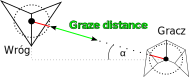
\includegraphics[width=0.5\textwidth]{./images/kolizje01}
				\end{center}
				Każdy obiekt gry posiada swojego tzw. hitboxa, elipsę lub koło, które wyznacza obszar zdarzeń obiektu. Podczas testowania kolizji algorytm oblicza:
				\begin{enumerate}
					\item Dystans i kąt pomiędzy wrogimi obiektami
					\item Dla każdego hitobxa dystans pomiędzy punktem środkowym, a punktem znajdującym się na linii zderzenia
					\item Jeżeli oba hitboxy są ze sobą styczne lub na siebie nachodzą, następuje kolizja
					\item Jeżeli nie doszło do kolizji, ale obiekt Gracza znajduje się w pewnej określonej odległości między wrogim obiektem, tak, że można powiedzieć, że się o niego "otarł", zdobywa dodatkowe punkty.
				\end{enumerate}
			\subsection{Kształt hitboxa}
				\begin{center}
					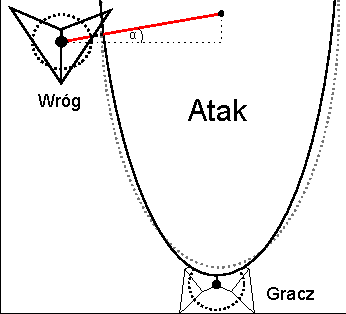
\includegraphics[width=0.4\textwidth]{./images/hitbox01}
				\end{center}
				Kształt naszego "pola zderzeń" nie jest stricte kołem, ale elipsą. Decyzja wynikła z tego, że w naszej grze będą duże, wypukłe obiekty dla których pole zderzeń w postaci koła może wyglądać nieatrakcyjnie. Dlatego zdecydowaliśmy się na elipsę, która dostosowuje wymiary swoich półosi do boków sprajta.
	
		\section{Zarządzanie zasobami}
			W naszych pierwszych krokach każdy obiekt gry posiadał osobny dla siebie sprajt. Nawet jeżeli wszystkie Pociski we Wzorze posiadały ten sam sprajt, każdy miał osobno przydzieloną pamięć. Powodowało to znaczne opóźnienia zarówno we wczytywaniu jak i podczas samej gry.\\\\
			Później zdecydowaliśmy się utworzyć nowy typ klas \textit{Resource}, które mapują i przechowują wskaźniki do utworzonych sprajtów. Z kolei każdy obiekt otrzymuje potrzebny wskaźnik, któremu jedynie przekazuje informację, w którym miejscu sprajt narysować. Każdy sprajt tworzony jest tylko raz oraz wyłącznie wtedy, gdy pojawia się na danej Planszy.\\\\
			Wyjątkami są te rodzaje sprajtów, które są niezbędne przez cały czas trwania gry:
			\begin{itemize}
				\item Bonusy, które mogą pojawić się w każdej chwili, ich kształt jest ściśle związany z typem
				\item Pociski Gracza, ich rodzaj zmienia się zależnie od zebranej mocy w czasie gry, każdy z nich może być potrzebny w dowolnym momencie. 
			\end{itemize}
			
		\section{Jednoczesne iterowanie i usuwanie z kolekcji}
			\begin{center}
				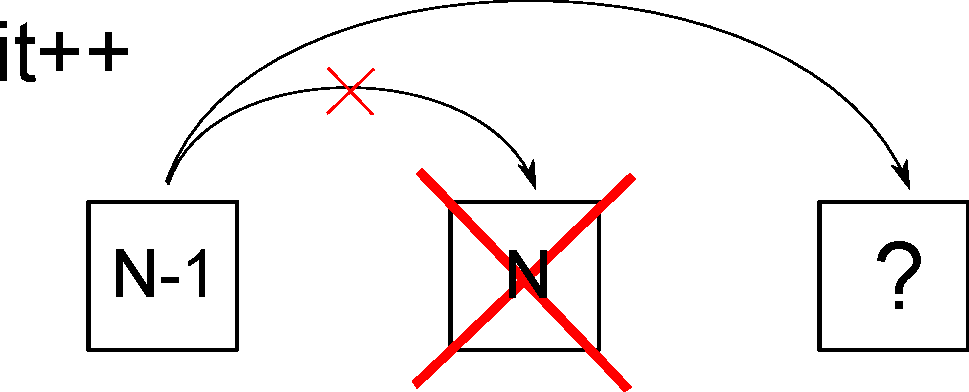
\includegraphics[width=0.6\textwidth]{./images/iteracja01}
			\end{center}
			Sprawdzanie kolizji odbywa się wg wielokrotnej iteracji. Np. każdy obiekt pocisku sprawdza czy występuje kolizja z każdym możliwym obiektem.
			\begin{itemize}
				\item Jeżeli kolizja nastąpiła:
				\begin{itemize}
					\item pocisk zostaje usunięty, a wrogi obiekt otrzymuje odpowiednie obrażenia.
					\item Jeżeli życia wroga tym samym spadło do zera, on również zostaje usunięty
				\end{itemize}
				\item Jeżeli kolizja nie nastąpiła, pociski dalej posuwa się swojej drogi
			\end{itemize}
			Jednakże może dojść do sytuacji w której usunięty pocisk lub wróg jest ostatnim z kolejki. Usunięcie odbywa się w trakcie pojedynczej iteracji, a po jej zakończeniu iterator jest inkrementowany. Po usunięciu ostatniego elementu iterator wskazuje na koniec kolejki, a po wyjściu z zakończeniu iteracji mechanizm chce by wskazał jeszcze dalej, bo powoduje błąd.\\\\
			Rozwiązaliśmy to przez dodanie dodatkowego warunku podczas iteracji, mianowicie, pod koniec iteracja jest sprawdzany warunek, czy iteracja jest możliwa (czyli czy nie został usunięty ostatni z kolejki). Wymaga to 2 razy więcej operacji typu IF, jednakże wygląda na to, że nie da się tego uniknąć. 
			
	
	\newpage
	\part{Podział pracy}
	
	
	
	
	
	
	
	
	
	
	
	
	
	
	
	
	
	
	
	
	
	
	
	
	
	
	
	
	
	
	
	
\end{document}